\documentclass{article}
\usepackage{FinalYearProjectReport}

% uncomment this line to double line spacing for proof reading
% \linespread{2}

% packages and settings for graphics
\usepackage[pdftex]{graphicx}
\graphicspath{{./}}
\DeclareGraphicsExtensions{.png}
\usepackage[final]{pdfpages}

\setlength\paperheight{297mm}
\setlength\paperwidth{210mm}

\usepackage{avant}
\renewcommand{\familydefault}{\sfdefault}
\frenchspacing

\title{Final Report}
\name{Alex \textsc{Andela}, Adil \textsc{Bhayani}, Vaishnavi \textsc{Muppavaram} \& Sakayan \textsc{Sitsabesan}}
\address{Department of Electrical and Computer Engineering\\
University of Auckland, Auckland, New Zealand}

\begin{document}

\begin{titlepage}

\newcommand{\HRule}{\rule{\linewidth}{0.5mm}}

\center
 
%----------------------------------------------------------------------------------------
%	HEADING SECTIONS
%----------------------------------------------------------------------------------------

\textsc{\LARGE University of Auckland}\\[1.5cm]
\textsc{\Large COMPSYS 301: Design: Hardware and Software Systems }\\[0.5cm]
\textsc{\large Autonomous Line Following Robot}\\[0.5cm]

%----------------------------------------------------------------------------------------
%	TITLE SECTION
%----------------------------------------------------------------------------------------

\HRule \\[0.4cm]
{ \huge \bfseries Final Report}\\[0.4cm]
\HRule \\[1.5cm]
 
%----------------------------------------------------------------------------------------
%	AUTHOR SECTION
%----------------------------------------------------------------------------------------

\begin{minipage}{0.4\textwidth}
\begin{flushleft} \large
\emph{Authors:}\\
Alex \textsc{Andela} \newline
Adil \textsc{Bhayani} \newline
Vaishnavi \textsc{Muppavaram} \newline
Sakayan \textsc{Sitsabesan}
\end{flushleft}
\end{minipage}
~
\begin{minipage}{0.4\textwidth}
\begin{flushright} \large
\emph{Supervisors:} \\
Dr. Nitish \textsc{Patel} \\
Dr. Muhammad \textsc{Nadeem} % Supervisor's Name
\end{flushright}
\end{minipage}\\[1cm]

%----------------------------------------------------------------------------------------
%	DATE SECTION
%----------------------------------------------------------------------------------------

{\large \today}\\[2cm]

%----------------------------------------------------------------------------------------
%	LOGO SECTION
%----------------------------------------------------------------------------------------


\includegraphics{uoa.png}\\[1cm]
 
%----------------------------------------------------------------------------------------

\vfill

\vspace*{25em}

{\Large Declaration of Originality}

\hspace{5em}

This report is our own unaided work and was not copied from nor written in collaboration with any other person.

Name: Alex \textsc{Andela}, Adil \textsc{Bhayani}, Vaishnavi \textsc{Muppavaram} \& Sakayan \textsc{Sitsabesan}

\newpage

{\Large Acknowledgments}

\hspace{5em}

We would like to thank our supervisors, Dr. Nitish Patel \& Dr. Muhammad Nadeem, for guiding us throughout the semester with their constant help, supervision and suggestions. We would also like to thank Fung Yang \& Howard Lu for their patience dealing with our numerous issues and changes with the robot hardware. Special mentions need to be made to Joseph Tsoi, Andrew Lai \& John Zhang for their ideas and assistance.

\end{titlepage}

\newpage

\maketitle

\begin{abstract}

The Mini Project consists of designing a game on a FPGA device which incorporates one simple tank defence game called Tank Hunting. The overall objective is to learn the process of digital design and logic by practically applying the skills learnt prior to the project.

\end{abstract}


%----------------------------------------------------------------------------------------
%	INTRODUCTION
%----------------------------------------------------------------------------------------

\section{Design Overview}

This project consisted of the design and construction of part of an autonomous line following robot, which will complete certain benchmarks and can pick up all the "food pellets" in a given map. Much of the robot's hardware was prescribed and given to us in an assembled state for working on. The sensor circuit was the only important part of the hardware that needed to be completed as part of this project. The robot was controlled from a Cypress PSoC 5LP, which interfaced with the Sensors, RF, Bluetooth \&  Motors to allow the robot to meet its requirements. This report outlines the hardware and software considerations and decisions that were made as part of this project.

\section{Robot Description}

%----------------------------------------------------------------------------------------
%	ANALOGUE SECION
%----------------------------------------------------------------------------------------
% Mention considerations and decisions here

\section{Analogue}

\subsection{Phototransistor output signal}

\subsection{Circuitry}

\subsection{Light sensor array and robot orientation}

\subsection{PCB Design}

\subsection{Testing and Verification}

\subsection{Final Design}

%----------------------------------------------------------------------------------------
%	DIGITAL SECION
%----------------------------------------------------------------------------------------
% Mention considerations and decisions here

\section{Digital}

\subsection{Path Finding Algorithms}

\subsection{Line Following}

\subsection{Motion Control \& PID}

\subsection{Block Diagram}

\begin{figure}[!h]
\centerline{
\includegraphics[width=0.5\textwidth]{uoa}}
\caption{Block Diagram}
\label{fig:rawFrame}
\end{figure}

\subsection{RF \& Bluetooth}

\subsection{Testing and Verification}

\subsection{Final Design}

\subsection{Data Structures}

%----------------------------------------------------------------------------------------
%	CONCLUSIONS
%----------------------------------------------------------------------------------------

\section{Conclusions}

\section{Contributions}

%----------------------------------------------------------------------------------------
%	APPENDICES
%----------------------------------------------------------------------------------------

\clearpage

\section{Appendices}

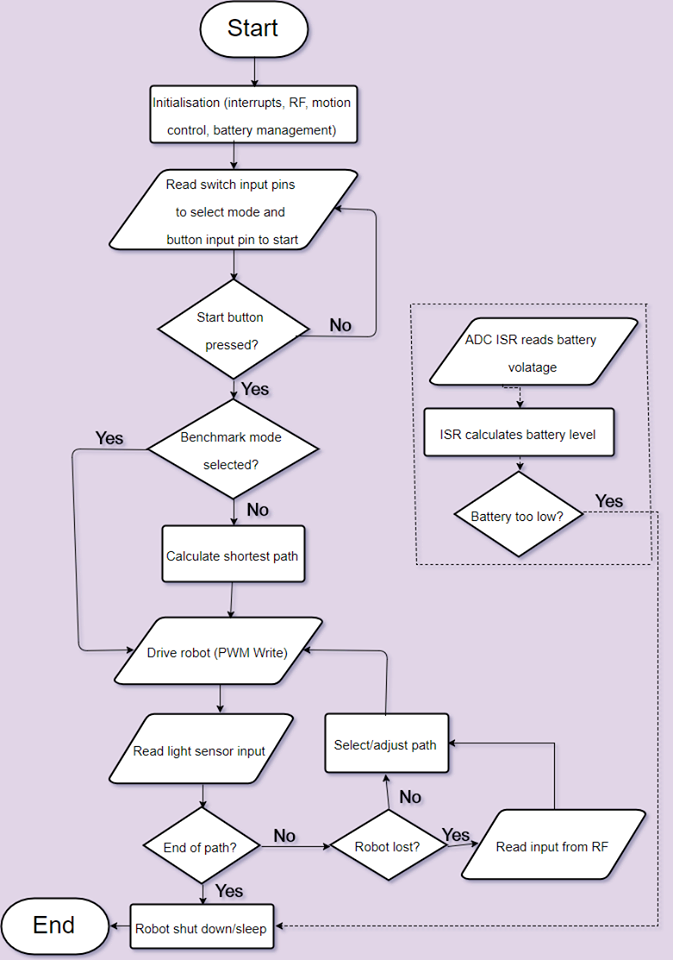
\includegraphics[width=0.5\textwidth]{software_flowchart.png}

\vfill

\end{document}